\documentclass[authoryear, review, 11pt]{elsarticle}

\setlength{\textwidth}{6.5in}
%\setlength{\textheight}{9in}
\setlength{\topmargin}{0in}
\setlength{\oddsidemargin}{0in}
\setlength{\evensidemargin}{0in}

\usepackage{amsmath}
\usepackage{amsthm}
\usepackage{amssymb}

\usepackage{bm}

%\geometry{landscape}                % Activate for for rotated page geometry
\usepackage[parfill]{parskip}    % Activate to begin paragraphs with an empty line rather than an indent
\usepackage{graphicx}
\usepackage{epstopdf}
\usepackage{natbib}

\usepackage{relsize}
\usepackage{subfigure}
%\usepackage{fullpage}
\usepackage{booktabs}

\DeclareGraphicsRule{.tif}{png}{.png}{`convert #1 `dirname #1`/`basename #1 .tif`.png}
\DeclareMathOperator*{\argmin}{\arg\!\min}
\DeclareMathOperator*{\argmax}{\arg\!\max}
\DeclareMathOperator*{\bw}{\mbox{bw}}
\DeclareMathOperator*{\df}{\mbox{df}}
\newcommand{\vect}[1]{\bm{#1}}
\newcommand{\E}{\mathop{\mathbb E}}


\title{GW-SELECT}
\author{Wesley Brooks}
\date{}                                           % Activate to display a given date or no date

\begin{document}
\maketitle
%\section{}
%\subsection{}





\section{Introduction}
	%Varying-coefficient regression is a technique used in spatial statistics to model a non-stationary process. Geographically Weighted Regression (GWR) \cite{Fotheringham:2002} is a method of fitting varying-coefficient models. 

	%The goal of this project is to develop a method that can answer these questions and work out the conditions under which the answers are reliable. Variable selection is via the Adaptive-LASSO, applied independently to each local model. The LASSO for GWR models was introduced in \cite{Wheeler:2009}. That paper describes a process for model fitting that is similar to our process in the case of Gaussian data, but does not cover the Generalized Linear Model (GLM) case for non-Gaussian data that nevertheless follows an exponential-family distribution. Justification for the process in \cite{Wheeler:2009} is by simulation - the paper does not present theoretical proof of consistency of its estimators nor does it prove an oracle property for its variable selection.\\
	
	%The method in \cite{Wheeler:2009} requires cross-validation to select the model's tuning parameter and thus local models can be built only at locations where the output variable has been observed. It will be desirable to build local models that interpolate between the locations where the observations were taken. Using an information criterion like the Akaike Information Criterion (AIC) or Bayesian Information Criterion (BIC) to select the tuning parameter could solve this problem. Another option is weighted cross-validation.\\

	
\section{Geographically-weighted regression models \label{section:model}}

	\subsection{Model}
	Consider $n$ data observations, made at locations $s_1, \dots, s_n$. For $i \in \left\{1, \dots, n \right\}$, let $y(s_i)$ and $\bm{x}(s_i)$ be the univariate outcome of interest, and a $(p+1)$-variate vector of covariates measured at location $s_i$, respectively.
	
	
	Consider $n$ observations of $(p+1)$-variate $\bm{X} = \left( \bm{x}(s_1), \dots, \bm{x}(s_n) \right)'$ and univariate $\bm{y} = \left( y(s_1), \dots, y(s_n) \right)$, where each observation is associated with a location $s_i$, $i \in \left\{ 1, \dots, n \right\}$ and let there exist a spatially-varying coefficient surface $\bm{\beta}(s)$ such that	
	\begin{eqnarray}
		y(s_i) = \bm{x}'(s_i) \bm{\beta}(s_i) + \epsilon(s_i)
	\end{eqnarray}
	
	where the error term $\epsilon(s)$ is normally distributed with zero mean and a possibly spatially-varying variance $\sigma^2(s)$:	
	\begin{eqnarray}
		\epsilon(s_i) \sim \mathcal{N} \left( 0,\sigma^2(s_i) \right)
	\end{eqnarray}
	
	In order to simplify the notation, let subscripts denote the values of data or parameters at the locations where data is observed. Thus, $\bm{x}(s_i) \equiv \bm{x}_i \equiv \left( 1, x_{i1}, \dots, x_{ip} \right)'$, $\bm{\beta}(s_i) \equiv \bm{\beta}_i \equiv \left(\beta_{i0}, \beta_{i1}, \dots, \beta_{ip} \right)'$, $y(s_i) \equiv y_i$, and $\sigma^2(s_i) \equiv \sigma^2_i$. Let $\bm{X} = \left( \bm{x}_1, \dots, \bm{x}_n \right)'$ and $\bm{Y} = \left( y_1, \dots, y_n \right)'$. The likelihood of the observed data is then	 
	 \begin{eqnarray}
	 	L\left( \bm{\beta} \right) = \prod_{i=1}^n \left[ \left(2 \pi \sigma^2_i\right)^{-\frac{1}{2}} \exp \left\{-\left( 2\sigma^2_i \right)^{-1} \left(y_i - \bm{x}'_i\bm{\beta}_i \right)^2 \right\} \right]
	\end{eqnarray}
	
	\subsection{Geographically-weighted regression}
	Geographically-weighted regression (GWR) estimates the value of the coefficient surface $\bm{\beta}(s)$ at each location $s_i$. Estimation is done by maximizing the local likelihood \citep{Fotheringham:2002}.	
	\begin{eqnarray}
		\ell_i\left(\bm{\beta}_i\right) &=& \sum_{i'=1}^n \left\{ -\frac{1}{2} \log{\left(2 \pi\right)}  - \frac{1}{2} \log{\left(\sigma^2_i w^{-2}_{ii'} \right)}  -\left( 2 \sigma^2_i w^{-2}_{ii'} \right)^{-1} \left(y_{i'} - \bm{x}'_{i'} \bm{\beta}_i \right)^2 \right\}
	\end{eqnarray}
	
	The first and second derivatives of the local log-likelihood are $\frac{\partial \ell_i}{\partial \bm{\beta}_i} =  \left\{ \sum_{i'=1}^n \left[ x_{i'j} \left( \sigma^2_i w^{-2}_{ii'} \right)^{-1} \left( y_{i'} - \bm{x}'_{i'} \bm{\beta}_i \right) \right] \right\}$ and 
	\begin{eqnarray}
		\frac{\partial^2 \ell_i}{\partial \bm{\beta}_i \partial \bm{\beta}'_i} = \left( \begin{array}{ccc} -\sum_{i'=1}^n \left\{ x^2_{i'1} \left( \sigma^2_i w^{-2}_{ii'} \right)^{-1} \right\}  & \cdots & -\sum_{i'=1}^n \left\{ x_{i'1} x_{i'p} \left( \sigma^2_i w^{-2}_{ii'} \right)^{-1} \right\} \\ \vdots & \ddots & \vdots \\ -\sum_{i'=1}^n \left\{ x_{i'p} x_{i'1} \left( \sigma^2_i w^{-2}_{ii'} \right)^{-1} \right\}  & \cdots & -\sum_{i'=1}^n \left\{ x^2_{i'p} \left( \sigma^2_i w^{-2}_{ii'} \right)^{-1} \right\} \end{array} \right)
	\end{eqnarray}
	
	So the observed Fisher information in the locally weighted sample is	
	\begin{eqnarray}
		\mathcal{J}_i = \sigma^{-2}_i \left( \begin{array}{ccc} \sum_{i'=1}^n \left( x_{i'1} w_{ii'} \right)^2 & \dots & \sum_{i'=1}^n \left\{ \left(x_{i'1} w_{ii'}\right) \left(x_{i'p} w_{ii'}\right) \right\} \\ \vdots & \ddots & \vdots \\ \sum_{i'=1}^n \left\{ \left(x_{i'p} w_{ii'}\right) \left(x_{i'1} w_{ii'}\right)  \right\} & \dots & \sum_{i'=1}^n \left( x_{i'p} w_{ii'} \right)^2 \end{array} \right)
	\end{eqnarray}	
	
	The bisquare kernel function is used to generate geographic weights based on the distance between observation locations. For estimating the value of the coefficient surface at location $s_i$, the weight given to the observation at location $s_{i'}$ is	
	\begin{eqnarray}
		w_{ii'} = \begin{cases} \left[ 1-\left( \bw^{-1} \|s_i-s_{i'}\| \right)^2 \right] & \mbox{ if } \|s_i-s_{i'}\| < \bw \\ 0 & \mbox{ if } \|s_i-s_{i'}\| \geq \bw \end{cases}
	\end{eqnarray}
	
	where $\bw$ is the kernel bandwidth.\\
	
	Letting the weight matrix $\bm{W}_i$ be	
	\begin{eqnarray}
		\bm{W}_i =  \left( \begin{array}{ccc} w_{i1} & \cdots & 0 \\ \vdots & \ddots & \vdots \\ 0 & \cdots & w_{in} \end{array} \right)
	\end{eqnarray}
	
	estimation of the ordinary geographically-weighted regression coefficient surface is by weighted least squares:	
	\begin{eqnarray}
		\hat{\bm{\beta}}_{i, \mbox{GWR}} = \left( \bm{X}'\bm{W}_i\bm{X} \right)^{-1} \bm{X}'\bm{W}_i\bm{Y}
	\end{eqnarray}
	
	
	At each location $s_i$, the ordinary geographically-weighted regression estimator minimizes the objective function:
	\begin{eqnarray}
		\sum_{i'=1}^n w_{ii'} \left(y_{i'} - \bm{x}'_{i'} \bm{\beta}_i \right)^2
	\end{eqnarray}
	
	 The estimated local variance $\hat{\sigma}_i^2$ is the variance estimate of the unpenalized local model \citep{Zou:2007}.
	
\section{Model selection and shrinkage \label{section:method}}
	Coefficient shrinkage and variable selection are accomplished locally via the Lasso \citep{Tibshirani:1996}.
	
	The objective minimized by the geographically-weighted also (GWL) is:	
	\begin{eqnarray}
		\sum_{i'=1}^n w_{ii'} \left(y_{i'} - \bm{x}'_{i'} \bm{\beta}_i \right)^2 + \sum_{j=1}^p \lambda_{ij} \beta_{ij}
	\end{eqnarray}
	
	Where $\lambda_{ij}, j \in \{1, \dots, p\}$ are penalties from the adaptive lasso \citep{Zou:2006}.\\
	
	The LAR algorithm is a stepwise regression algorithm; the number of steps to include in the model is chosen by minimizing the local AIC, with the sum of the weights around$s_i$ $\sum_{i'=1}^n w_{ii'}$ playing the role of the sample size and the number of nonzero coefficients in $\bm{\beta}_i$ playing the role of the ``degrees of freedom" $\left( \df_i \right)$ \citep{Zou:2007}.

	Thus:
	\begin{eqnarray}
		\mbox{AIC}_{\mbox{loc}} = \sum_{i'=1}^n w_{ii'} \hat{\sigma}_i^{-2} \left( y_{i'} - \bm{x}'_{i'} \hat{\bm{\beta}}_i \right)^2 + 2 \mbox{df}_i
	\end{eqnarray}

	Because GWL is not a linear smoother (there is no smoothing matrix $\bm{S}$ such that $\hat{\bm{y}} = \bm{S} \bm{y}$) the AIC and confidence intervals as calculated in \cite{Fotheringham:2002} are not accurate for the GWL \citep{Zou:2006}.

	\subsection{Bandwidth selection}
		The bandwidth is selected to minimize the total AIC. Because of the kernel weights and the application of the lasso, the sample size and degrees of freedom are different for each observation. The total AIC is found by taking the sum over all of the observed data:		
		\begin{eqnarray}
			\mbox{AIC}_{\mbox{tot}} = \sum_{i=1}^n \left( \hat{\sigma}_i^{-2} \left( y_i - \bm{x}'_i \hat{\bm{\beta}}_i \right)^2 + \log \hat{\sigma}_i^2 + 2 \mbox{df}_i \left(\sum_{i'=1}^n w_{ii'} \right)^{-1} \right)
		\end{eqnarray}
			
			The bandwidth that minimizes $\mbox{AIC}_{\mbox{tot}}$ is found by a line search.\\
			
\section{Simulation}
	\subsection{Simulation setup}
		A simulation study was conducted to assess the finite-sample properties of the method described in Sections \ref{section:model}-\ref{section:method}. Data was simulated on $[0,1] \times [0,1]$, which was divided into a $30 \times 30$ grid. Each of the $p=5$ covariates was simulated by a Gaussian random field with mean zero and exponential covariance $Cov \left(Z_j(s_i), Z_j(s_{i'}) \right) = \sigma^2 \exp{\left( -\tau^{-1} \|s_i - s_{i'} \| \right)}$ where $\sigma^2=1$ is the variance and $\tau$ is a range parameter. Correlation was induced between the covariates by multiplying the $\bm{Z}$ matrix by the Cholesky decomposition of the covariance matrix $\Sigma = \bm{R}'\bm{R}$. The covariance matrix is a $5 \times 5$ matrix that has ones on the diagonal and $\rho$ for all off-diagonal entries, where $\rho$ is the between-covariate correlation.\\
		
		The simulated response is $Y(s) = \bm{X}(s) \bm{\beta}(s) + \epsilon(s)$, where the coefficient surface used to generate the data is $\bm{\beta}(s) = \left( \beta_0(s), \dots, \beta_5(s) \right) = \left( 0, \beta_1(s), 0, 0, 0, 0 \right)$ and $\epsilon(s) \overset{\mbox{iid}}{\sim} \mathcal{N} \left( 0, 1 \right)$.\\
		
		In order to evaluate the performance over a range of data conditions, the data was simulated at low and high values of the spatial covariance range, and at low and high values of the between-covariate correlation, for two cases of $\beta_1(s)$: the step function		
		\begin{eqnarray}
			\beta_1(s) = \begin{cases} 0 &\mbox{ if } s_y<0.5 \\ 1 &\mbox{ o.w.} \end{cases}
		\end{eqnarray}
		
		and the constant gradient $\beta_1(s) = 1-s_y$.
			
		Each case was simulated 100 times.\\
	
	\subsection{Simulation results}
		The coverage of the $95\%$ CI and the selection frequency are plotted in the figures.\\
		
		
			\begin{figure}
				\begin{center}
					\subfigure[Coverage of 95\% CI for $X_1$]{
						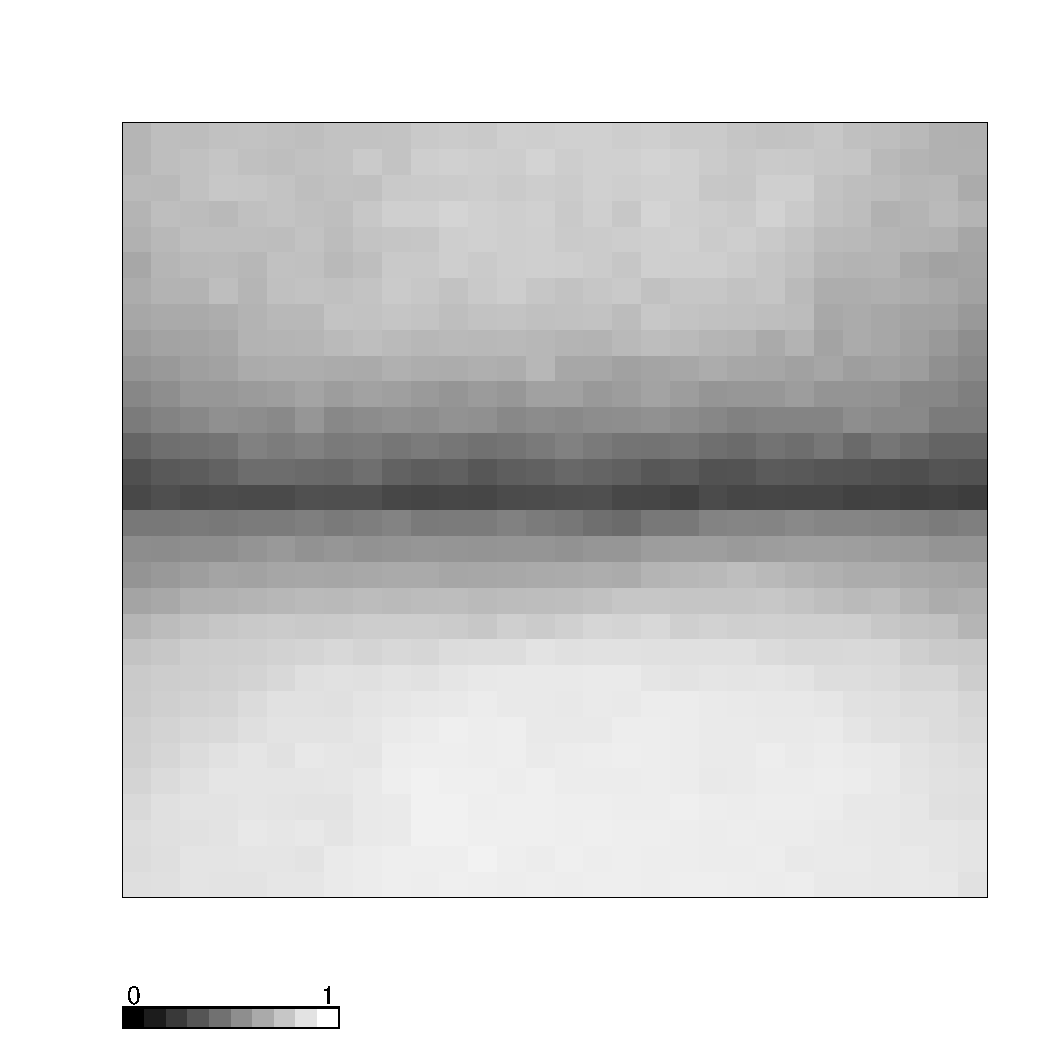
\includegraphics[width=3.1in]{../../figures/simulation/X1.coverage.pdf}
						\label{figX1:subfig1}
					}
					\subfigure[Selection frequency for $X_1$]{
						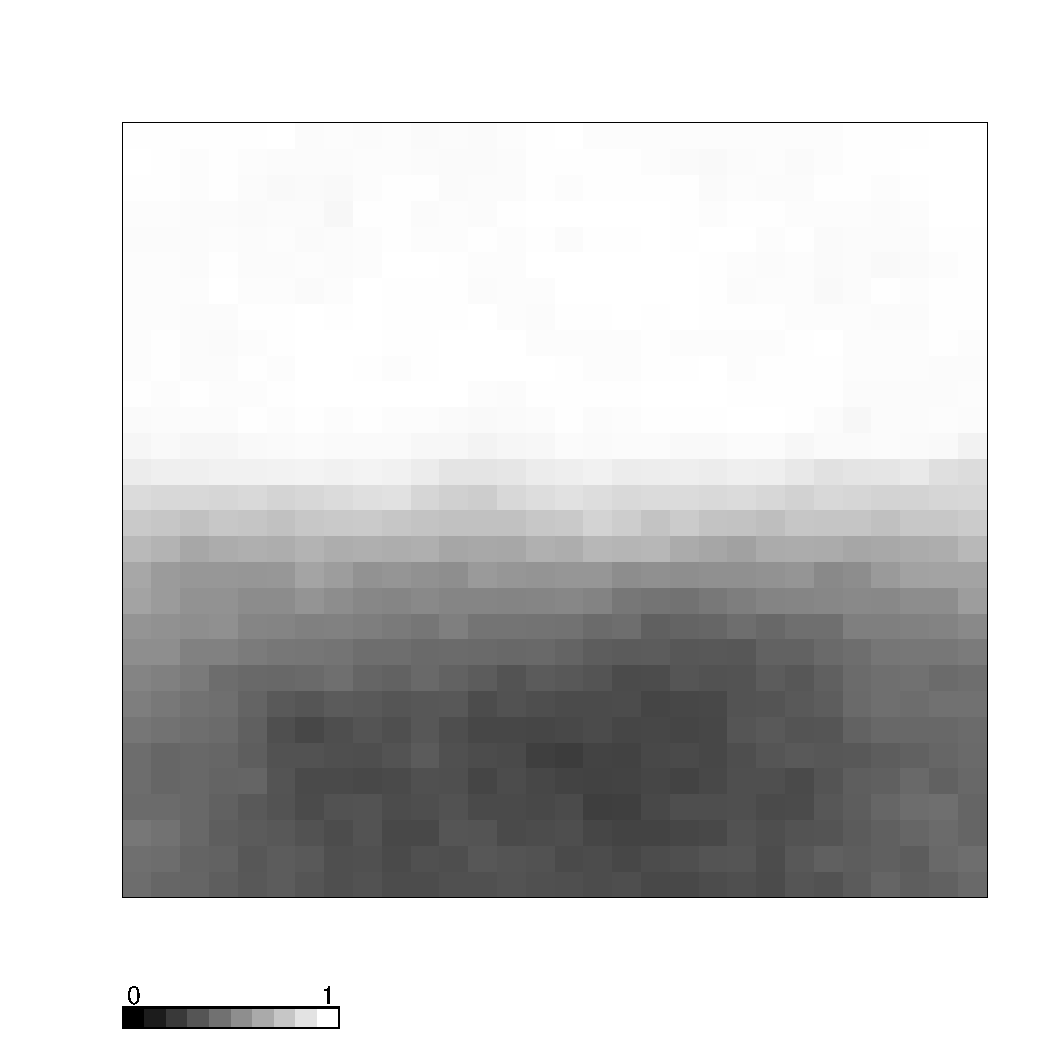
\includegraphics[width=3.1in]{../../figures/simulation/X1.selection.pdf}
						\label{figX1:subfig2}
					}
					\caption{Confidence interval coverage and selection frequency for $X_1$.\label{figX1}}
				\end{center}
			\end{figure}
					
					
			\begin{figure}
				\begin{center}
					\subfigure[Coverage of 95\% CI for $X_2$]{
						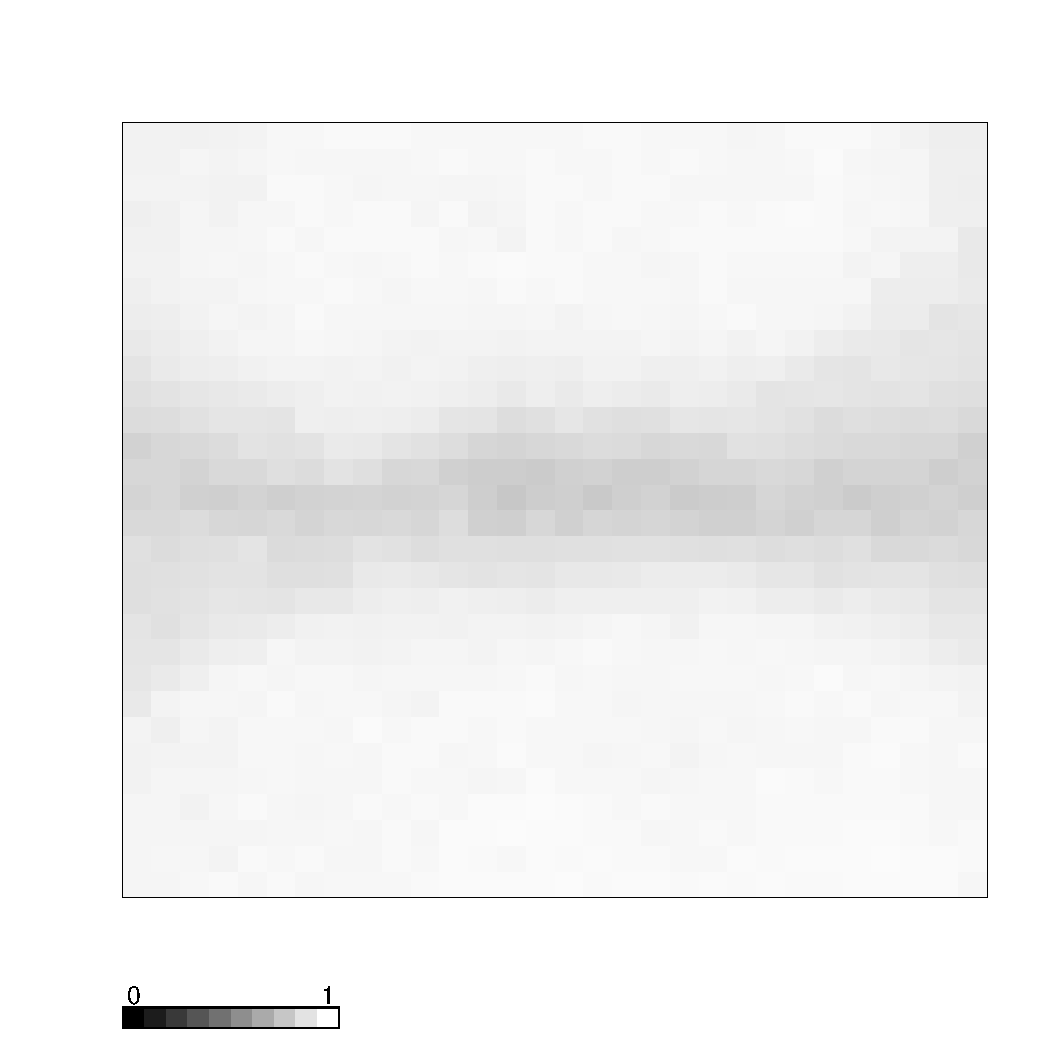
\includegraphics[width=3.1in]{../../figures/simulation/X2.coverage.pdf}
						\label{figX2:subfig1}
					}
					\subfigure[Selection frequency for $X_2$]{
						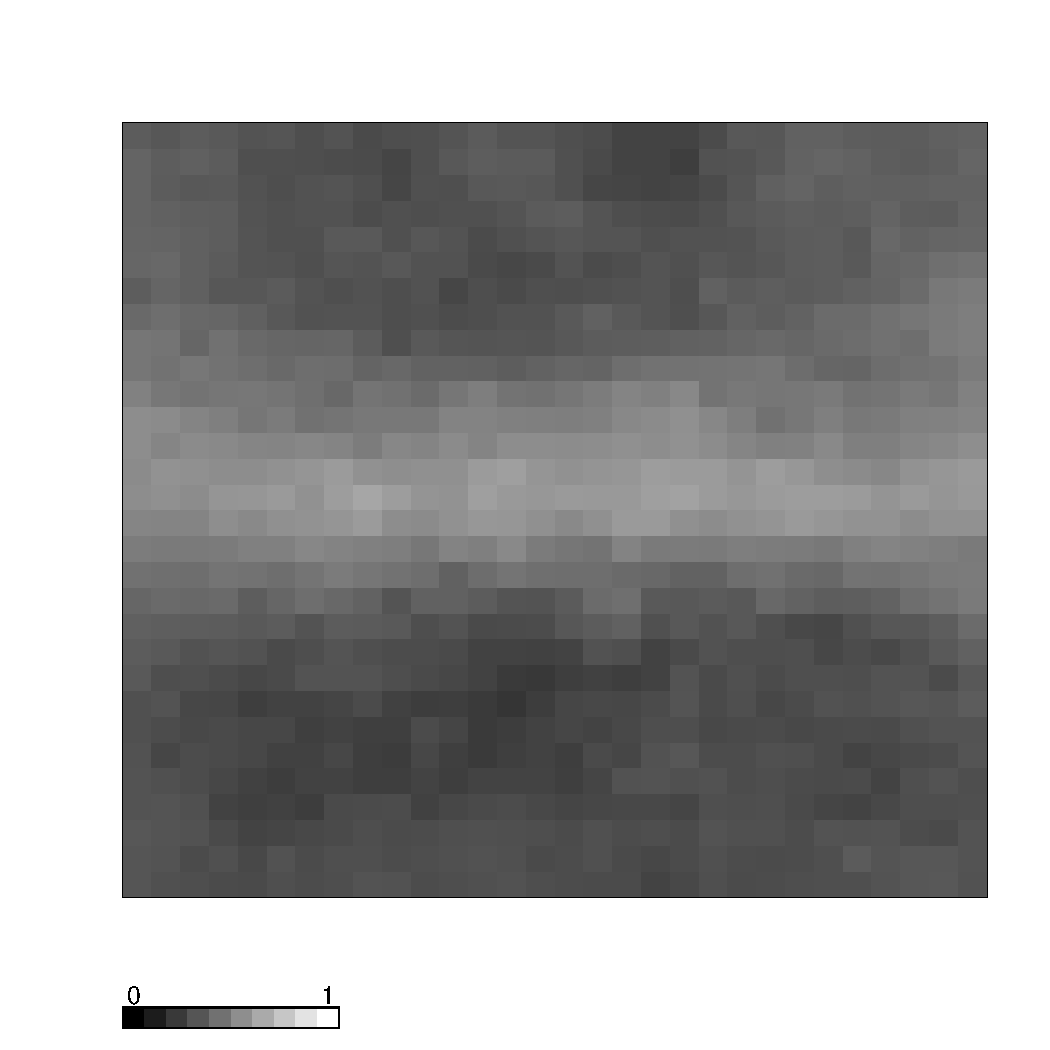
\includegraphics[width=3.1in]{../../figures/simulation/X2.selection.pdf}
						\label{figX2:subfig2}
					}									
					\caption{Confidence interval coverage and selection frequency for $X_2$.\label{figX2}}
				\end{center}
			\end{figure}
			
			
			\begin{figure}
				\begin{center}
					\subfigure[Coverage of 95\% CI for $X_3$]{
						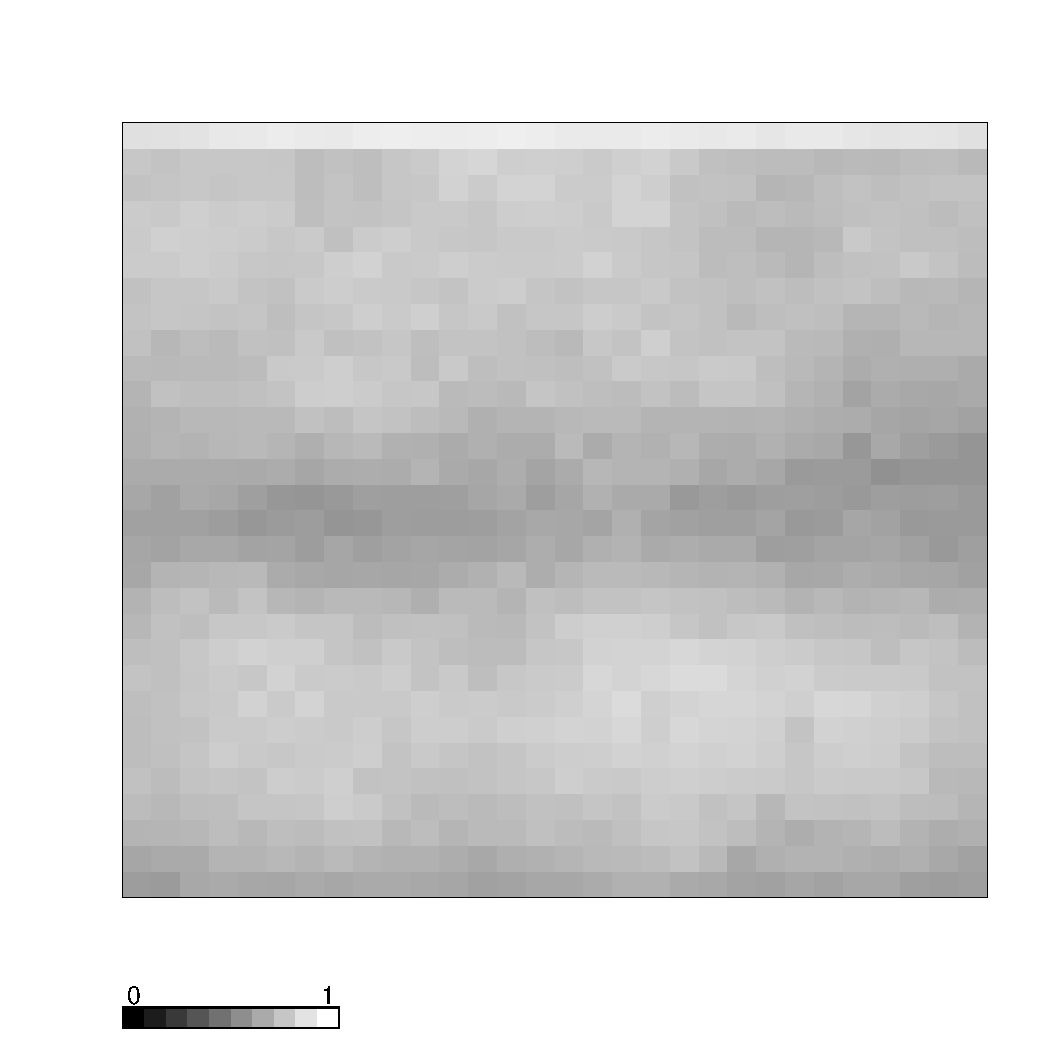
\includegraphics[width=3.1in]{../../figures/simulation/X3.coverage.pdf}
						\label{figX3:subfig1}
					}
					\subfigure[Selection frequency for $X_3$]{
						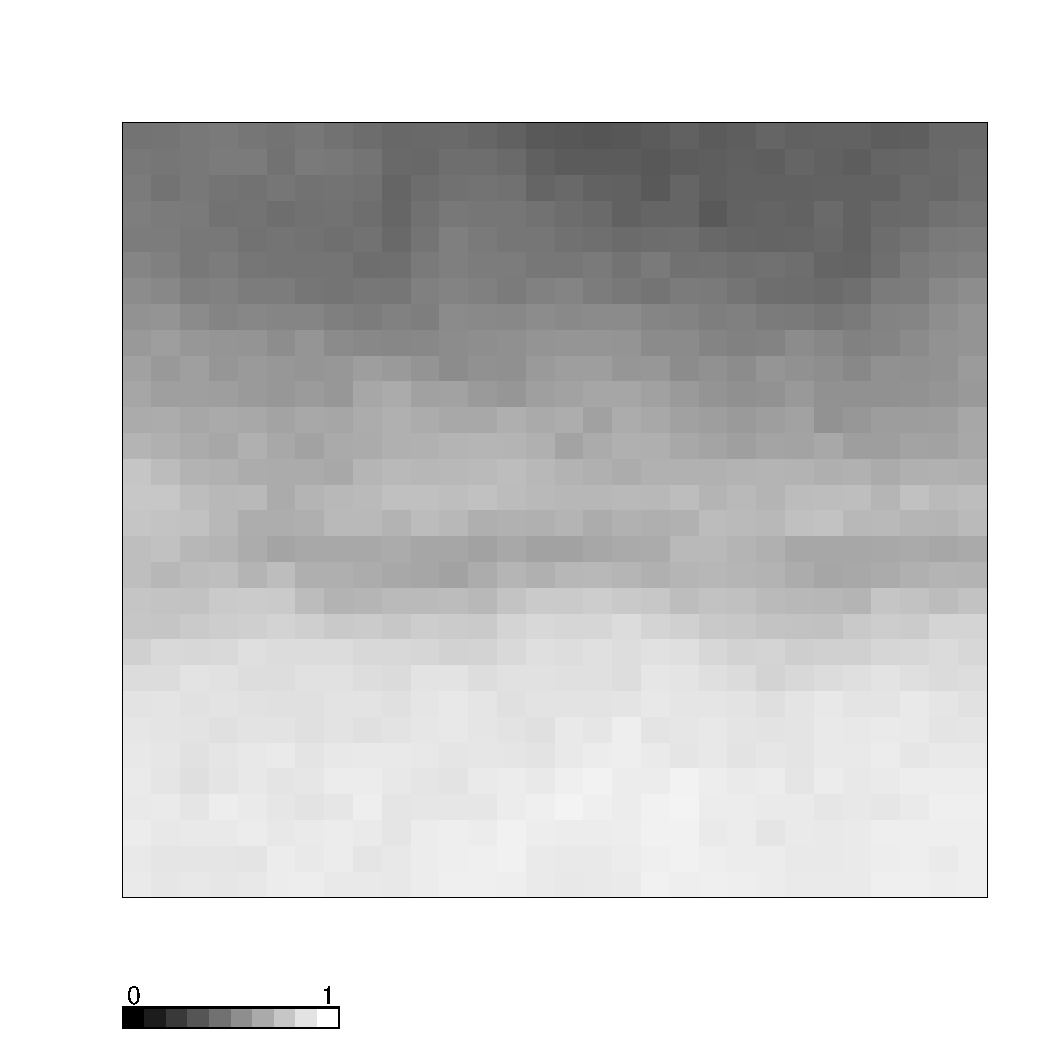
\includegraphics[width=3.1in]{../../figures/simulation/X3.selection.pdf}
						\label{figX3:subfig2}
					}									
					\caption{Confidence interval coverage and selection frequency for $X_3$.\label{figX3}}
				\end{center}
			\end{figure}
			
			
			\begin{figure}
				\begin{center}
					\subfigure[Coverage of 95\% CI for $X_4$]{
						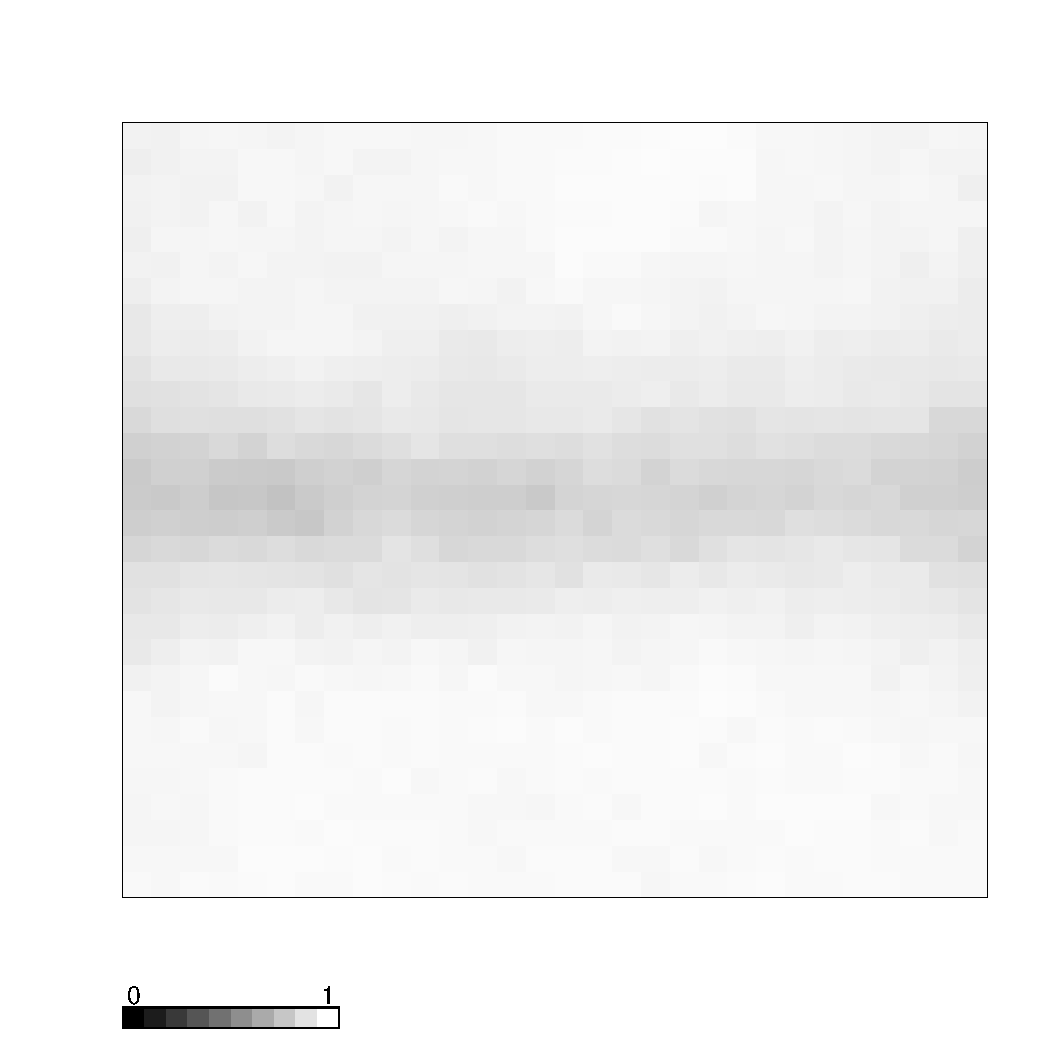
\includegraphics[width=3.1in]{../../figures/simulation/X4.coverage.pdf}
						\label{figX4:subfig1}
					}
					\subfigure[Selection frequency for $X_4$]{
						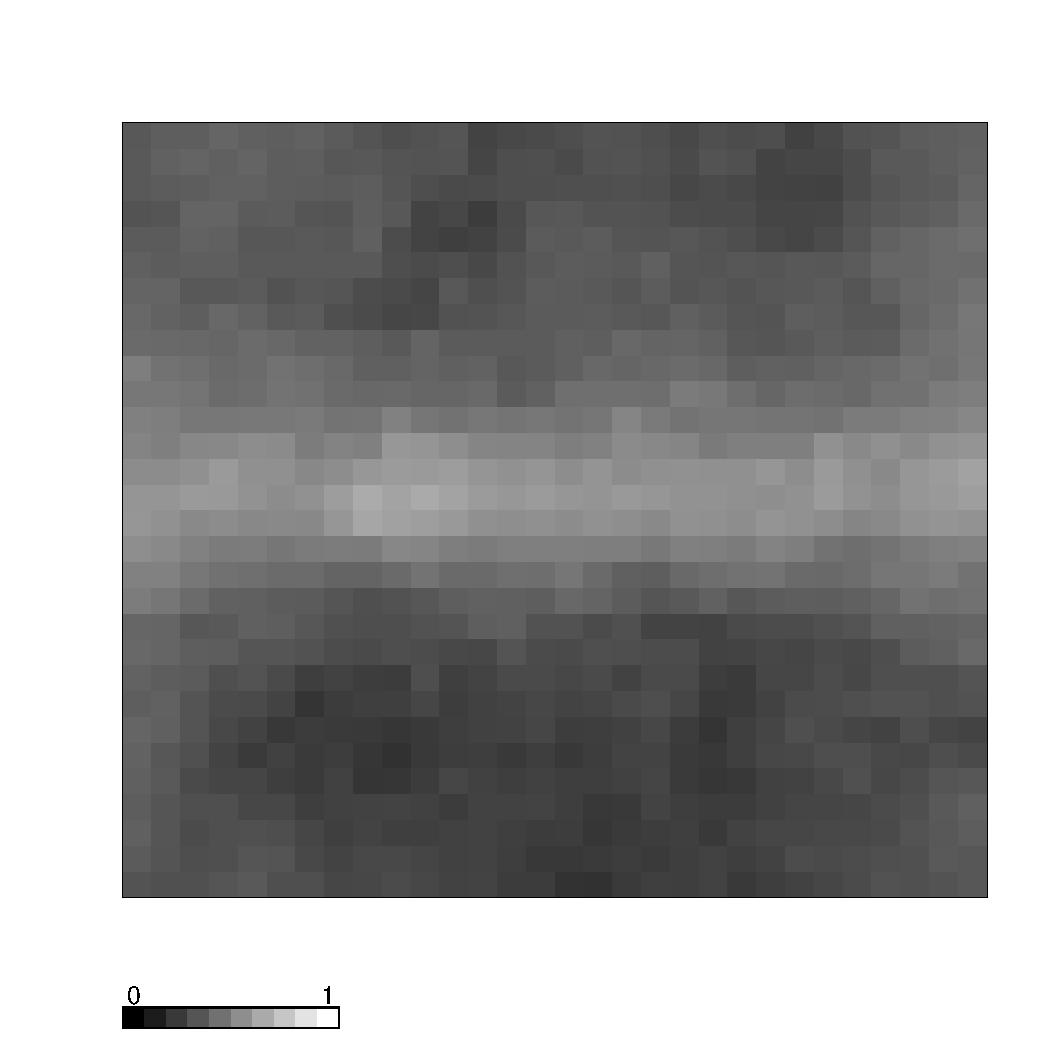
\includegraphics[width=3.1in]{../../figures/simulation/X4.selection.pdf}
						\label{figX4:subfig2}
					}									
					\caption{Confidence interval coverage and selection frequency for $X_4$.\label{figX4}}
				\end{center}
			\end{figure}
			
			
			\begin{figure}
				\begin{center}
					\subfigure[Coverage of 95\% CI for $X_5$]{
						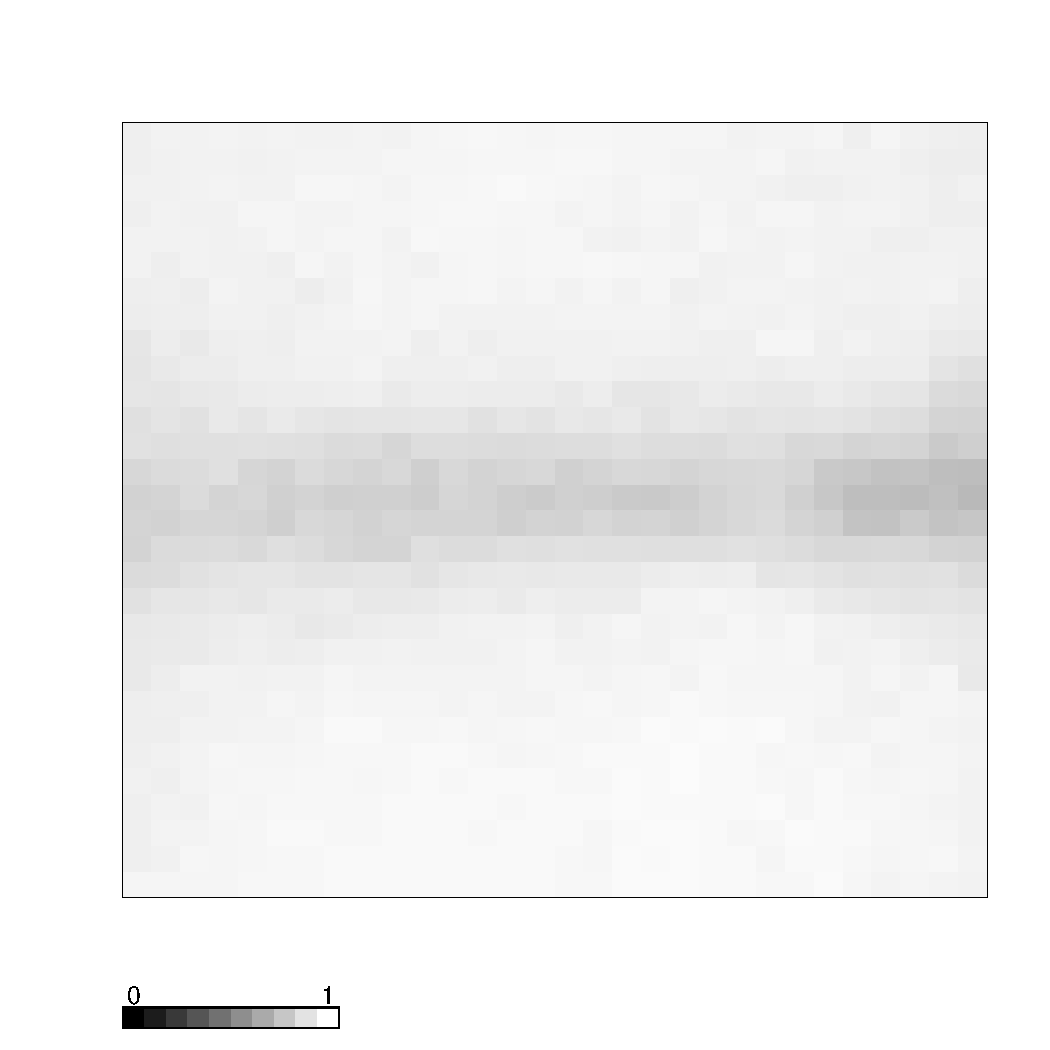
\includegraphics[width=3.1in]{../../figures/simulation/X5.coverage.pdf}
						\label{figX5:subfig1}
					}
					\subfigure[Selection frequency for $X_5$]{
						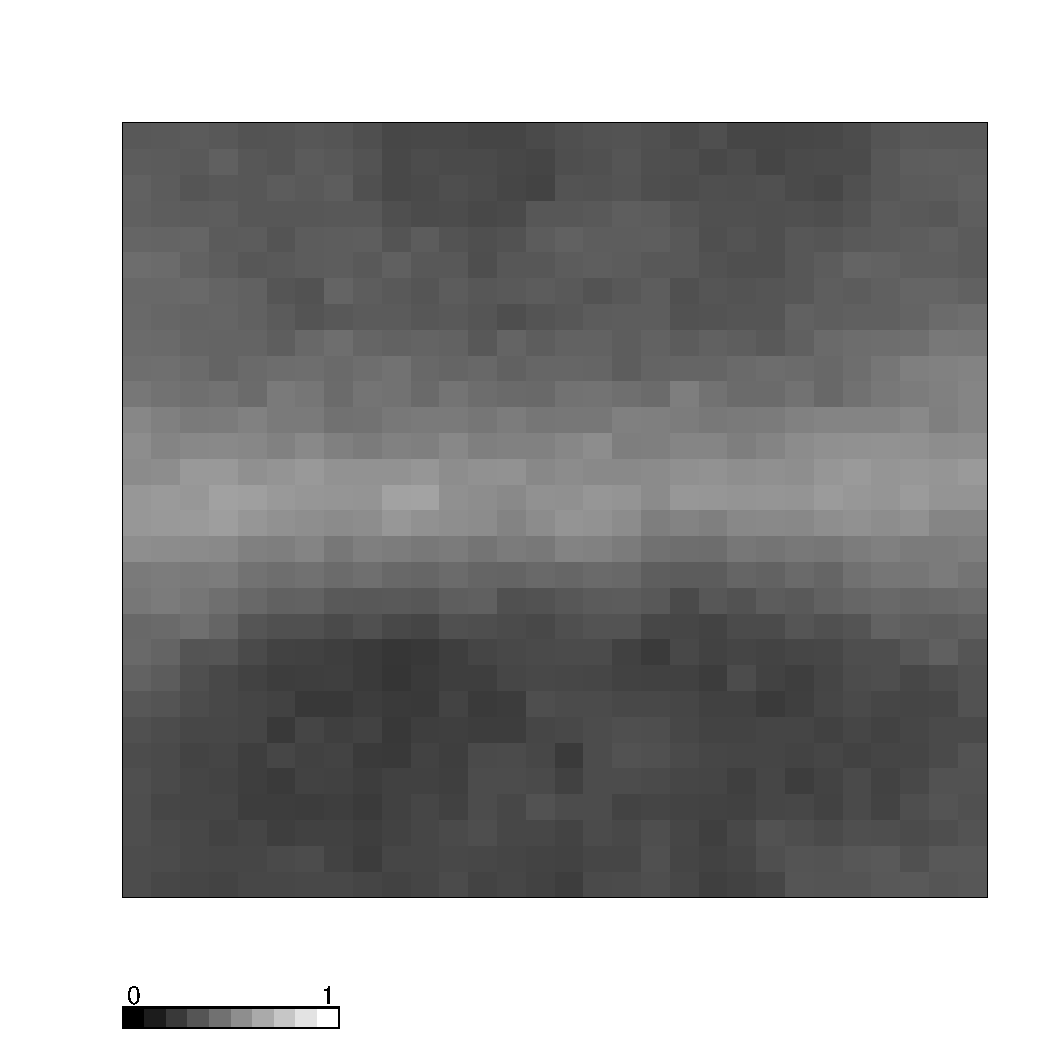
\includegraphics[width=3.1in]{../../figures/simulation/X5.selection.pdf}
						\label{figX5:subfig2}
					}									
					\caption{Confidence interval coverage and selection frequency for $X_5$.\label{figX5}}
				\end{center}
			\end{figure}
			
			
			\begin{figure}
				\begin{center}
					\subfigure[Coverage of 95\% CI for $Z$]{
						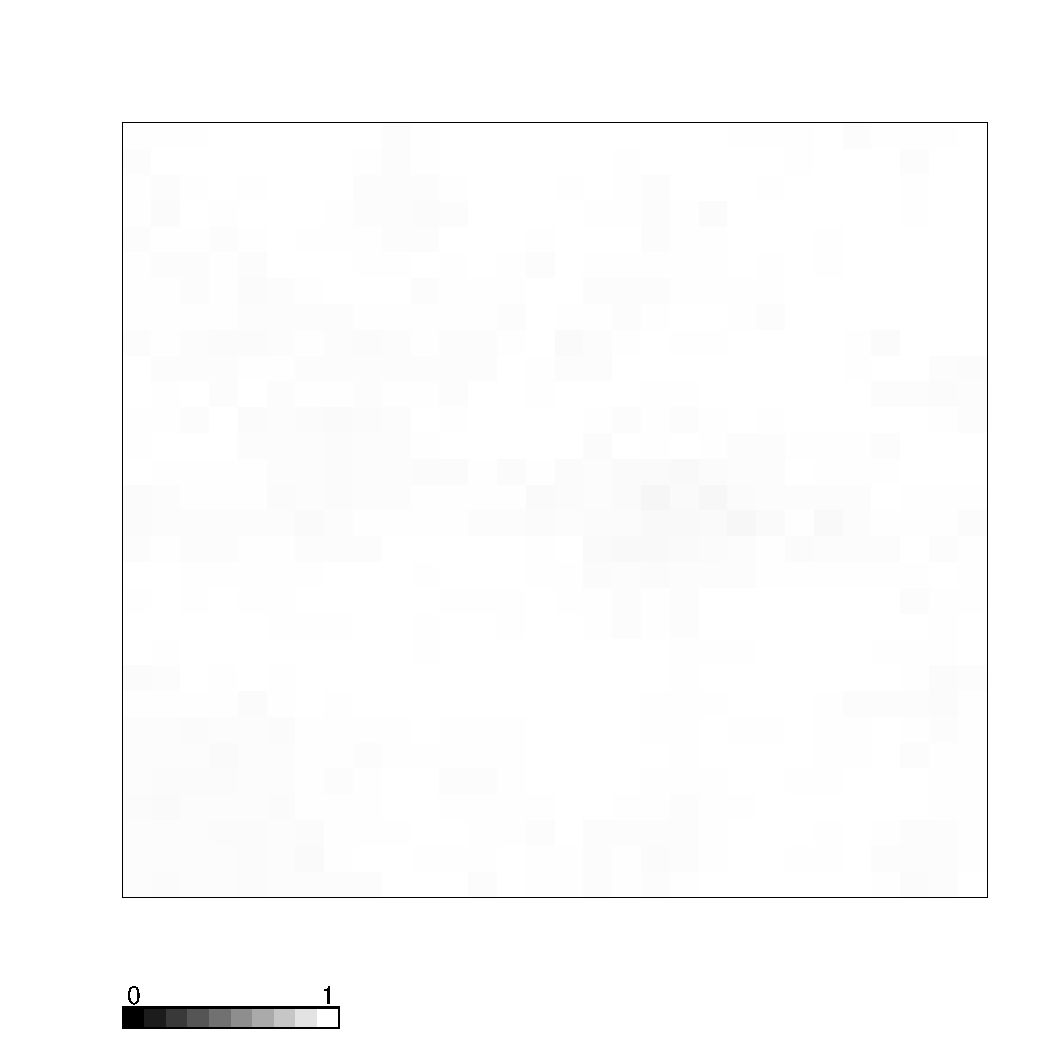
\includegraphics[width=3.1in]{../../figures/simulation/Z.coverage.pdf}
						\label{figZ:subfig1}
					}
					\subfigure[Selection frequency for $Z$]{
						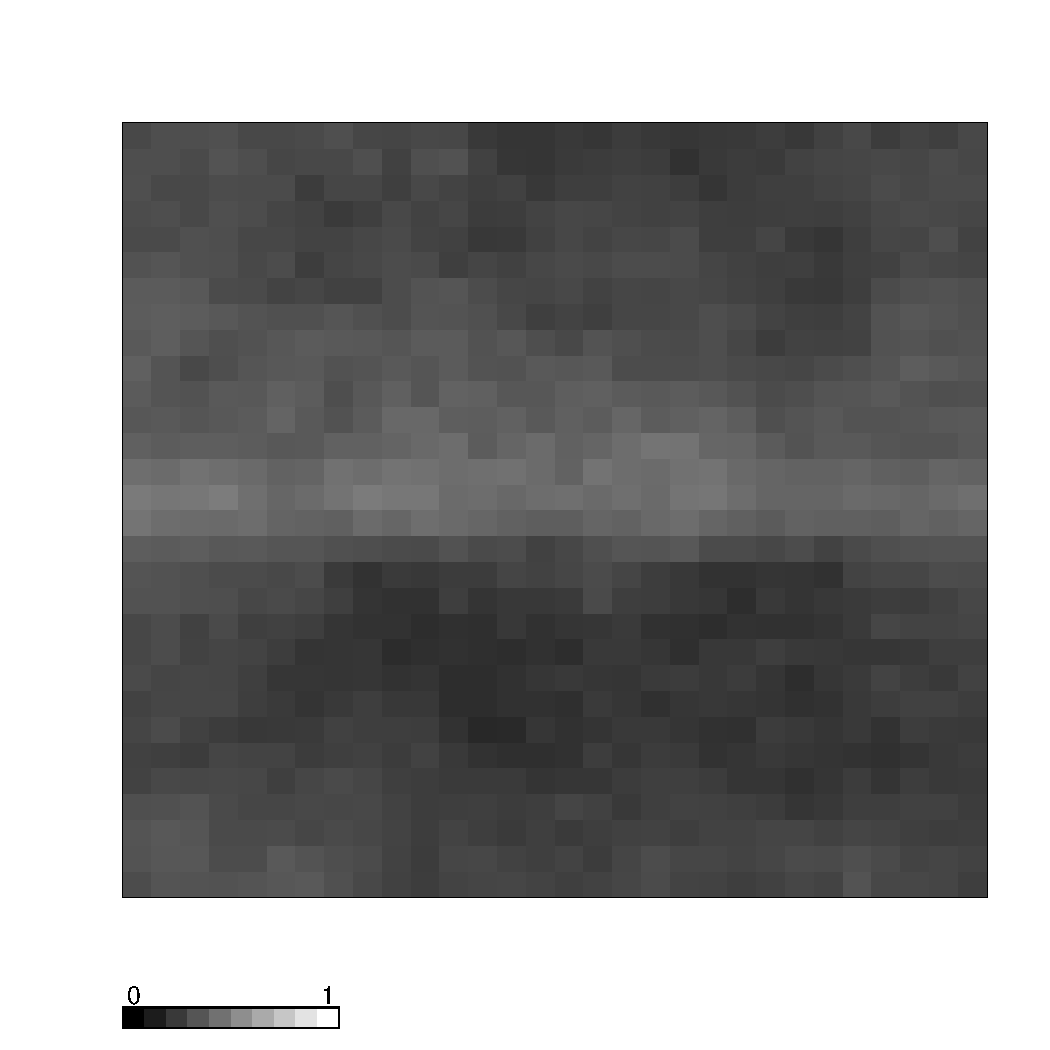
\includegraphics[width=3.1in]{../../figures/simulation/Z.selection.pdf}
						\label{figZ:subfig2}
					}									
					\caption{Confidence interval coverage and selection frequency for $Z$.\label{figZ}}
				\end{center}
			\end{figure}
			
			
			\begin{figure}
				\begin{center}
					\subfigure[Coverage of 95\% CI for intercept]{
						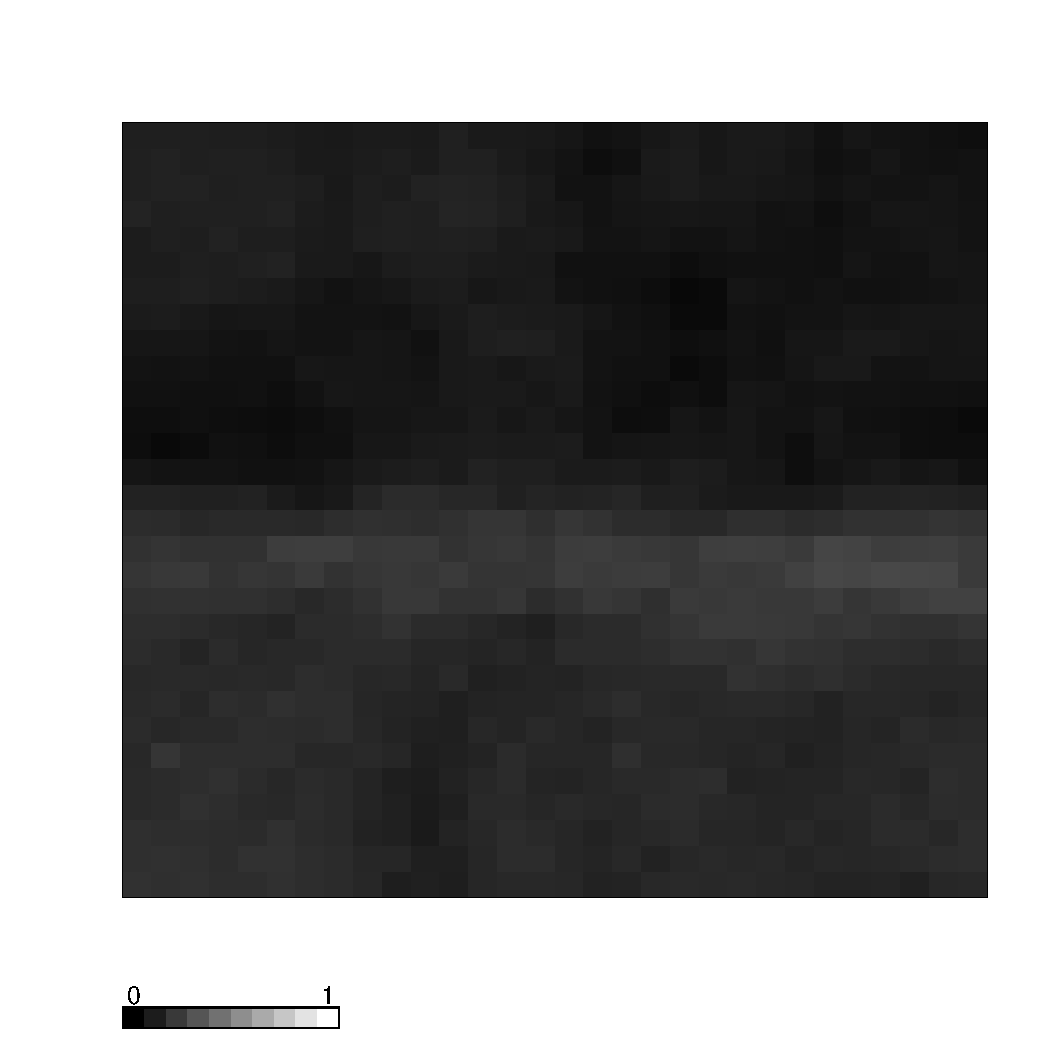
\includegraphics[width=3.1in]{../../figures/simulation/Intercept.coverage.pdf}
						\label{figIntercept:subfig1}
					}
					\subfigure[Selection frequency for intercept]{
						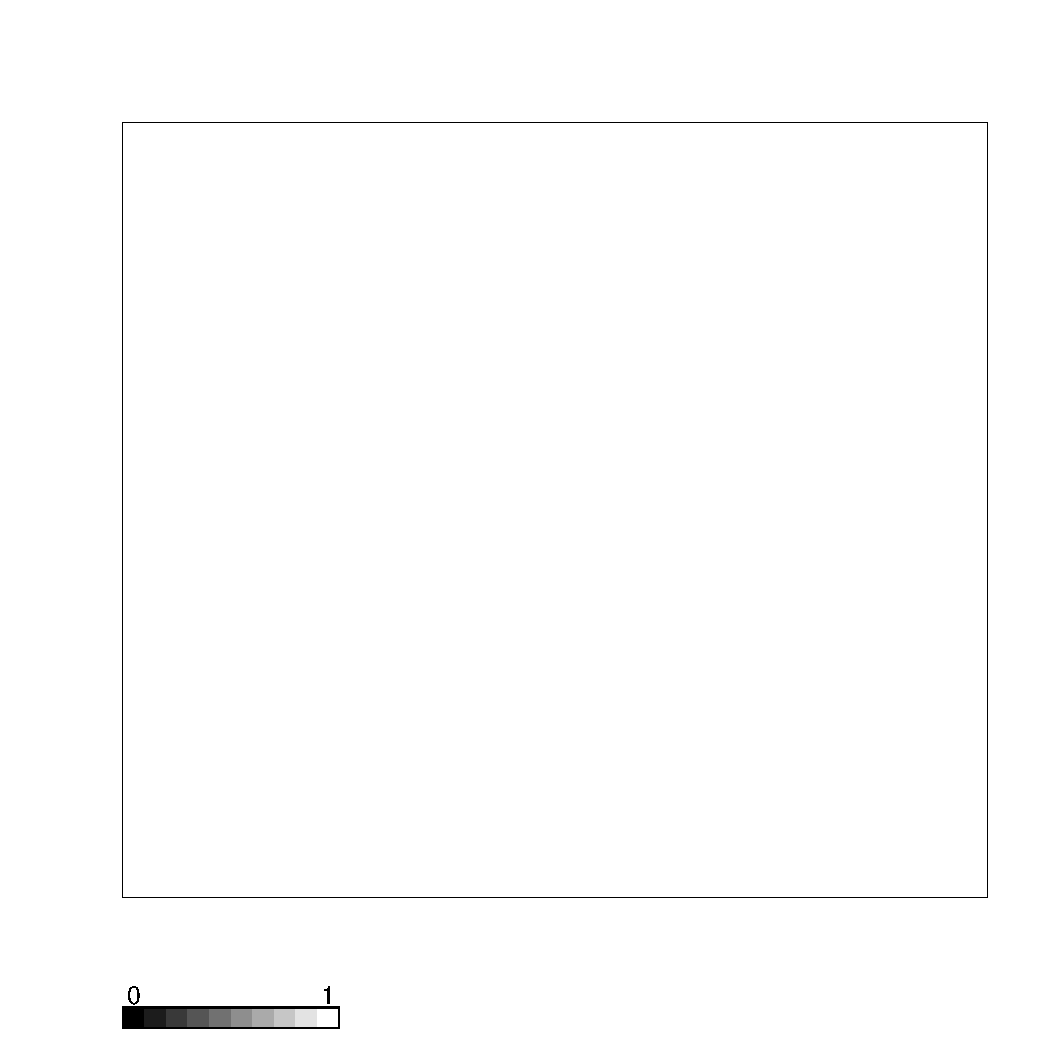
\includegraphics[width=3.1in]{../../figures/simulation/Intercept.selection.pdf}
						\label{figIntercept:subfig2}
					}									
					\caption{Confidence interval coverage and selection frequency for intercept.\label{figIntercept}}
				\end{center}
			\end{figure}
			
			
			
			
			
		%\subsection{Poverty data}
		%	\begin{figure}
		%		\begin{center}
		%			\includegraphics[width=5in]{../../figures/poverty/pag.estimate.pdf}
		%			\caption{Estimated coefficient surface for pag.\label{fig:pag}}
		%		\end{center}
		%	\end{figure}
		%			
		%			
		%	\begin{figure}
		%		\begin{center}
		%			\includegraphics[width=5in]{../../figures/poverty/pex.estimate.pdf}
		%			\caption{Estimated coefficient surface for pex.\label{fig:pex}}
		%		\end{center}
		%	\end{figure}
		%				
		%	
		%	\begin{figure}
		%		\begin{center}
		%			\includegraphics[width=5in]{../../figures/poverty/pman.estimate.pdf}
		%			\caption{Estimated coefficient surface for pman.\label{fig:pman}}
		%		\end{center}
		%	\end{figure}
		%				
		%	
		%	\begin{figure}
		%		\begin{center}
		%			\includegraphics[width=5in]{../../figures/poverty/pserve.estimate.pdf}
		%			\caption{Estimated coefficient surface for pserve.\label{fig:pserve}}
		%		\end{center}
		%	\end{figure}
		%				
		%	
		%	\begin{figure}
		%		\begin{center}
		%			\includegraphics[width=5in]{../../figures/poverty/pfire.estimate.pdf}
		%			\caption{Estimated coefficient surface for pfire.\label{fig:pfire}}
		%		\end{center}
		%	\end{figure}
		%				
		%	
		%	\begin{figure}
		%		\begin{center}
		%			\includegraphics[width=5in]{../../figures/poverty/potprof.estimate.pdf}
		%			\caption{Estimated coefficient surface for potprof.\label{fig:potprof}}
		%		\end{center}
		%	\end{figure}
		%	
		%	
		%	
		%	\begin{figure}
		%		\begin{center}
		%			\includegraphics[width=5in]{../../figures/poverty/pwh.estimate.pdf}
		%			\caption{Estimated coefficient surface for pwh.\label{fig:pwh}}
		%		\end{center}
		%	\end{figure}
		%				
		%	
		%	\begin{figure}
		%		\begin{center}
		%			\includegraphics[width=5in]{../../figures/poverty/pblk.estimate.pdf}
		%			\caption{Estimated coefficient surface for pblk.\label{fig:pblk}}
		%		\end{center}
		%	\end{figure}
		%				
		%	
		%	\begin{figure}
		%		\begin{center}
		%			\includegraphics[width=5in]{../../figures/poverty/phisp.estimate.pdf}
		%			\caption{Estimated coefficient surface for phisp.\label{fig:phisp}}
		%		\end{center}
		%	\end{figure}
		%				
		%	
		%	\begin{figure}
		%		\begin{center}
		%			\includegraphics[width=5in]{../../figures/poverty/metro.estimate.pdf}
		%			\caption{Estimated coefficient surface for metro.\label{fig:metro}}
		%		\end{center}
		%	\end{figure}
			


			
\section{References}
\bibliographystyle{chicago}
\bibliography{../../references/gwr}

\end{document}  